\documentclass[11pt,onecolumn,letterpaper]{article}

% -------------------- PAQUETES --------------------
\usepackage[utf8]{inputenc}
\usepackage[T1]{fontenc}
\usepackage{lmodern}
\usepackage{amsmath,amssymb}
\usepackage{graphicx}
\usepackage{booktabs,array}
\usepackage{float}
\usepackage{caption}
\usepackage{enumitem}
\usepackage{indentfirst}
\usepackage{setspace}
\usepackage{listings}
\usepackage[round,authoryear]{natbib}
\usepackage[colorlinks=true,allcolors=blue]{hyperref}
\usepackage{fancyhdr}
\usepackage{xcolor}
\usepackage[protrusion=true,expansion=false]{microtype}
\usepackage[letterpaper,left=1.25cm,right=1.25cm,top=2.50cm,bottom=2.50cm]{geometry}

% -------------------- FORMATO GENERAL --------------------
\setlist[itemize]{noitemsep,topsep=2pt,parsep=0pt,partopsep=0pt}
\setlist[enumerate]{noitemsep,topsep=2pt,parsep=0pt,partopsep=0pt}
\setlength{\parindent}{0.75cm}
\setlength{\parskip}{0pt}
\setlength{\headheight}{16pt}
\setlength{\emergencystretch}{2em}
\setlength{\jot}{5pt}
\setlength{\abovedisplayskip}{7pt}
\setlength{\belowdisplayskip}{7pt}
\setlength{\abovedisplayshortskip}{4pt}
\setlength{\belowdisplayshortskip}{4pt}
\onehalfspacing
\renewcommand{\arraystretch}{1.20}
\renewcommand{\thesection}{\Alph{section}}
\raggedbottom

\captionsetup[figure]{labelfont=bf,textfont=it,skip=8pt}
\captionsetup[table]{labelfont=bf,skip=8pt}
\renewcommand{\figurename}{Figura}
\renewcommand{\tablename}{Tabla}
\renewcommand{\contentsname}{Índice}
\renewcommand{\lstlistingname}{Código}
\renewcommand{\bibsection}{\section{Referencias}}

\definecolor{codegray}{RGB}{240,240,240}
\lstset{
    basicstyle=\ttfamily\small,
    backgroundcolor=\color{codegray},
    frame=single,
    rulecolor=\color{black!35},
    breaklines=true,
    showstringspaces=false,
    columns=fullflexible
}

\hypersetup{
    pdftitle={Control de Calidad en el Tratamiento Térmico de Piezas Mecánicas},
    pdfauthor={Biniza Verónica Vázquez Moreno, Joaquín Rosales González y Flor Denisse Hinojosa Hernández},
    pdfsubject={Avance uno de situación problema}
}

\newcommand{\Tamb}{T_{\mathrm{amb}}}
\newcommand{\Tsegura}{T_{\mathrm{segura}}}

% -------------------- PORTADA: ESTILO DEL EJEMPLO DE PRISM --------------------
\title{
    \vspace{0.8in}
    \IfFileExists{logo tec.png}{
\includegraphics[width=0.30\textwidth]{logo tec.png}\\\vspace{0.4cm}}{}
    \normalfont \normalsize \textsc{Avance uno de SP} \\ [10pt]
    \huge Control de Calidad en el Tratamiento Térmico \\
    \Large Modelación del enfriamiento de una pieza mecánica
}

\author{
Biniza Verónica Vázquez Moreno\\
Matrícula: A01737294\\[0.20cm]
Joaquín Rosales González\\
Matrícula: A01771481\\[0.20cm]
Flor Denisse Hinojosa Hernández\\
Matrícula: A00843678\\[0.30cm]
\small Modelación Matemática con Ecuaciones Diferenciales (MA1033.106)\\
\small Instituto Tecnológico y de Estudios Superiores de Monterrey
}

\date{31 de agosto de 2026}

% -------------------- ENCABEZADOS Y PIES --------------------
\pagestyle{fancy}
\fancyhf{}
\fancyhead[L]{Avance uno de SP}
\fancyhead[R]{Control de calidad en tratamiento térmico}
\fancyfoot[L]{Tecnológico de Monterrey}
\fancyfoot[R]{\thepage}
\renewcommand{\headrulewidth}{0.4pt}
\renewcommand{\footrulewidth}{0.4pt}

\begin{document}

\hypersetup{pageanchor=false}
\pagenumbering{roman}
\maketitle
\thispagestyle{empty}
\clearpage

\tableofcontents
\thispagestyle{empty}
\clearpage

\hypersetup{pageanchor=true}
\pagenumbering{arabic}

\section{Datos de identificación}

\begin{table}[H]
    \centering
    \begin{tabular}{@{}>{\bfseries}p{0.25\textwidth}p{0.67\textwidth}@{}}
        \toprule
        Institución & Tecnológico de Monterrey \\
        Unidad de Formación & Modelación Matemática con Ecuaciones Diferenciales (MA1033.106) \\
        Situación problema & Control de Calidad en el Tratamiento Térmico de Piezas Mecánicas \\
        Organización del caso & Mecánica Avanzada S.A. \\
        Integrantes & Biniza Verónica Vázquez Moreno, Joaquín Rosales González y Flor Denisse Hinojosa Hernández \\
        \bottomrule
    \end{tabular}
\end{table}

\section{Introducción y contextualización}

\subsection{Contexto y objetivo}

En este ejercicio se modeló el enfriamiento de un eje de acero después de salir del horno de templado. La pieza comienza a \(97\,^{\circ}\mathrm{C}\) y se deja enfriar en un taller que se mantiene a \(18\,^{\circ}\mathrm{C}\). Para manipularla, se toma \(27\,^{\circ}\mathrm{C}\) como temperatura segura.

Se buscó obtener el coeficiente de enfriamiento \(k\) a partir de 21 temperaturas simuladas, registradas cada
minuto durante los primeros 20 minutos. Con ese valor se construyó la función \(T(t)\), se calculó el tiempo necesario para llegar a \(27\,^{\circ}\mathrm{C}\) y se comprobó el resultado resolviendo la ecuación diferencial. También se analizó qué cambia si el taller está a \(24\,^{\circ}\mathrm{C}\).

\subsection{Variables, supuestos y método}

\begin{table}[H]
    \centering
    \caption{Variables utilizadas en el modelo.}
    \begin{tabular}{@{}p{0.27\textwidth}p{0.14\textwidth}p{0.53\textwidth}@{}}
        \toprule
        Elemento & Símbolo & Uso en el modelo \\
        \midrule
        Tiempo & \(t\) & Variable independiente medida en minutos. \\
        Temperatura & \(T(t)\) & Temperatura de la pieza en grados Celsius. \\
        Temperatura ambiente & \(\Tamb\) & Parámetro constante, inicialmente igual a \(18\,^{\circ}\mathrm{C}\). \\
        Coeficiente de enfriamiento & \(k\) & Constante positiva medida en \(\mathrm{min}^{-1}\). \\
        Condición inicial & \(T(0)\) & Temperatura inicial de \(97\,^{\circ}\mathrm{C}\). \\
        Temperatura segura & \(\Tsegura\) & Temperatura objetivo de \(27\,^{\circ}\mathrm{C}\). \\
        \bottomrule
    \end{tabular}
\end{table}

Se usó la ley de enfriamiento de Newton porque relaciona la rapidez de enfriamiento con la diferencia entre la temperatura de la pieza y la del ambiente \citep{incropera2017}. Para aplicarla, se supone que el taller conserva una temperatura constante, que \(T(t)\) representa una temperatura promedio de todo el eje y que \(k\) no cambia durante la prueba.

Primero se linealizaron los datos con \(\ln(T-\Tamb)\) para estimar \(k\). Después se resolvió la ecuación diferencial con la condición inicial exacta y se compararon los tiempos para verificar que ambos procedimientos describan el mismo enfriamiento.

\section{Desarrollo}

\subsection{Datos registrados}

Buscamos obtener el coeficiente de enfriamiento \(k\) a partir de 21 temperaturas
simuladas\footnote{Los datos fueron generados con asistencia de Claude
(Anthropic, 2025), a partir de una curva de enfriamiento exponencial con
\(k \approx 0.164\,\text{min}^{-1}\) y ruido aleatorio de \(\pm 0.2\)–\(0.5\,^{\circ}\mathrm{C}\)
para simular variabilidad realista de un pirómetro óptico.}, registradas cada
minuto durante los primeros 20 minutos.

\begin{table}[H]
    \centering
    \caption{Datos simulados usados para modelar el enfriamiento.}
    \label{tab:datos}
    \begin{tabular}{@{}rr@{\hspace{2.1cm}}rr@{}}
        \toprule
        \multicolumn{2}{c}{Mediciones 0--10 min} & \multicolumn{2}{c}{Mediciones 11--20 min} \\
        \cmidrule(r){1-2}\cmidrule(l){3-4}
        Tiempo (min) & \(T\) (\(^{\circ}\mathrm{C}\)) & Tiempo (min) & \(T\) (\(^{\circ}\mathrm{C}\)) \\
        \midrule
         0 & 97.0 & 11 & 31.3 \\
         1 & 85.4 & 12 & 28.9 \\
         2 & 74.6 & 13 & 27.6 \\
         3 & 66.8 & 14 & 25.8 \\
         4 & 58.7 & 15 & 24.9 \\
         5 & 53.1 & 16 & 23.6 \\
         6 & 47.3 & 17 & 22.8 \\
         7 & 43.6 & 18 & 22.0 \\
         8 & 39.0 & 19 & 21.4 \\
         9 & 36.4 & 20 & 20.6 \\
        10 & 33.1 &    &      \\
        \bottomrule
    \end{tabular}
\end{table}

Los datos originales se encuentran en \texttt{documentation/datos\_registrados.csv}.

\subsection{Regresión lineal y modelo numérico}

La ley de enfriamiento de Newton se expresa mediante la ecuación diferencial

\begin{equation}
    \frac{dT}{dt}=-k\left(T-\Tamb\right).
    \label{eq:newton}
\end{equation}

Su solución tiene forma exponencial:

\begin{equation*}
    T(t)-\Tamb=Ce^{-kt}.
\end{equation*}

No ajustamos una recta directamente a \(T(t)\), porque eso supondría que la pieza pierde la misma cantidad de grados cada minuto. Los datos muestran lo contrario: el descenso es rápido al principio y se hace menor cuando la pieza se acerca a \(18\,^{\circ}\mathrm{C}\). Restamos la temperatura ambiente para trabajar con el exceso de temperatura y aplicamos logaritmo natural; con esa transformación, la curva exponencial queda representada como una recta.

\begin{align*}
    \ln\left(T(t)-\Tamb\right)
        &=\ln\left(Ce^{-kt}\right) \\
        &=\ln(C)-kt.
\end{align*}

Si tomamos \(y=\ln(T-\Tamb)\) y \(x=t\), obtenemos la forma \(y=mx+b\). La pendiente es \(m=-k\), así que el coeficiente buscado es \(k=-m\); la intersección es \(b=\ln(C)\).

Hicimos esta operación con \texttt{analysis/modelo\_lineal.py}. El fragmento que transforma los datos y ejecuta la regresión es:

\begin{lstlisting}[language=Python,caption={Fragmento usado para linealizar los datos y obtener la recta.},label={lst:regresion}]
y_lin = np.log(T - Tm)
m, intercepto, r, p, error_estandar = stats.linregress(t, y_lin)
k_num = -m
C_num = np.exp(intercepto)
r_cuadrada = r**2
\end{lstlisting}

El CSV, el script completo y las gráficas se incluyen con la entrega. La recta obtenida fue

\begin{equation*}
    \ln(T-18)=-0.166700t+4.388000,
\end{equation*}

de donde obtenemos

\begin{align*}
    k_{\mathrm{num}} &= 0.166700\ \mathrm{min}^{-1}, \\
    C_{\mathrm{num}} &= e^{4.388000}=80.4793\,^{\circ}\mathrm{C}, \\
    R^2 &= 0.999206.
\end{align*}

El valor \(R^2=0.999206\) significa que la recta explica cerca del \(99.92\,\%\) de la variación de \(\ln(T-18)\) en estos 21 datos. Es un ajuste muy cercano, pero no prueba por sí solo que el modelo describa cualquier proceso de templado; solo indica qué tan bien funciona la relación linealizada para este conjunto simulado.

Vale la pena señalar una consideración estadística sobre este procedimiento: ajustar una recta sobre una variable linealizada mediante logaritmos introduce un sesgo de escala. La transformación logarítmica comprime las diferencias cuando \(T\) está lejos de \(\Tamb\) (mediciones iniciales) y las amplifica cuando \(T\) se acerca a \(\Tamb\) (mediciones finales), de modo que los puntos donde la pieza ya está casi fría pesan proporcionalmente más en el ajuste de la recta que los puntos iniciales.

\begin{figure}[htbp]
    \centering
    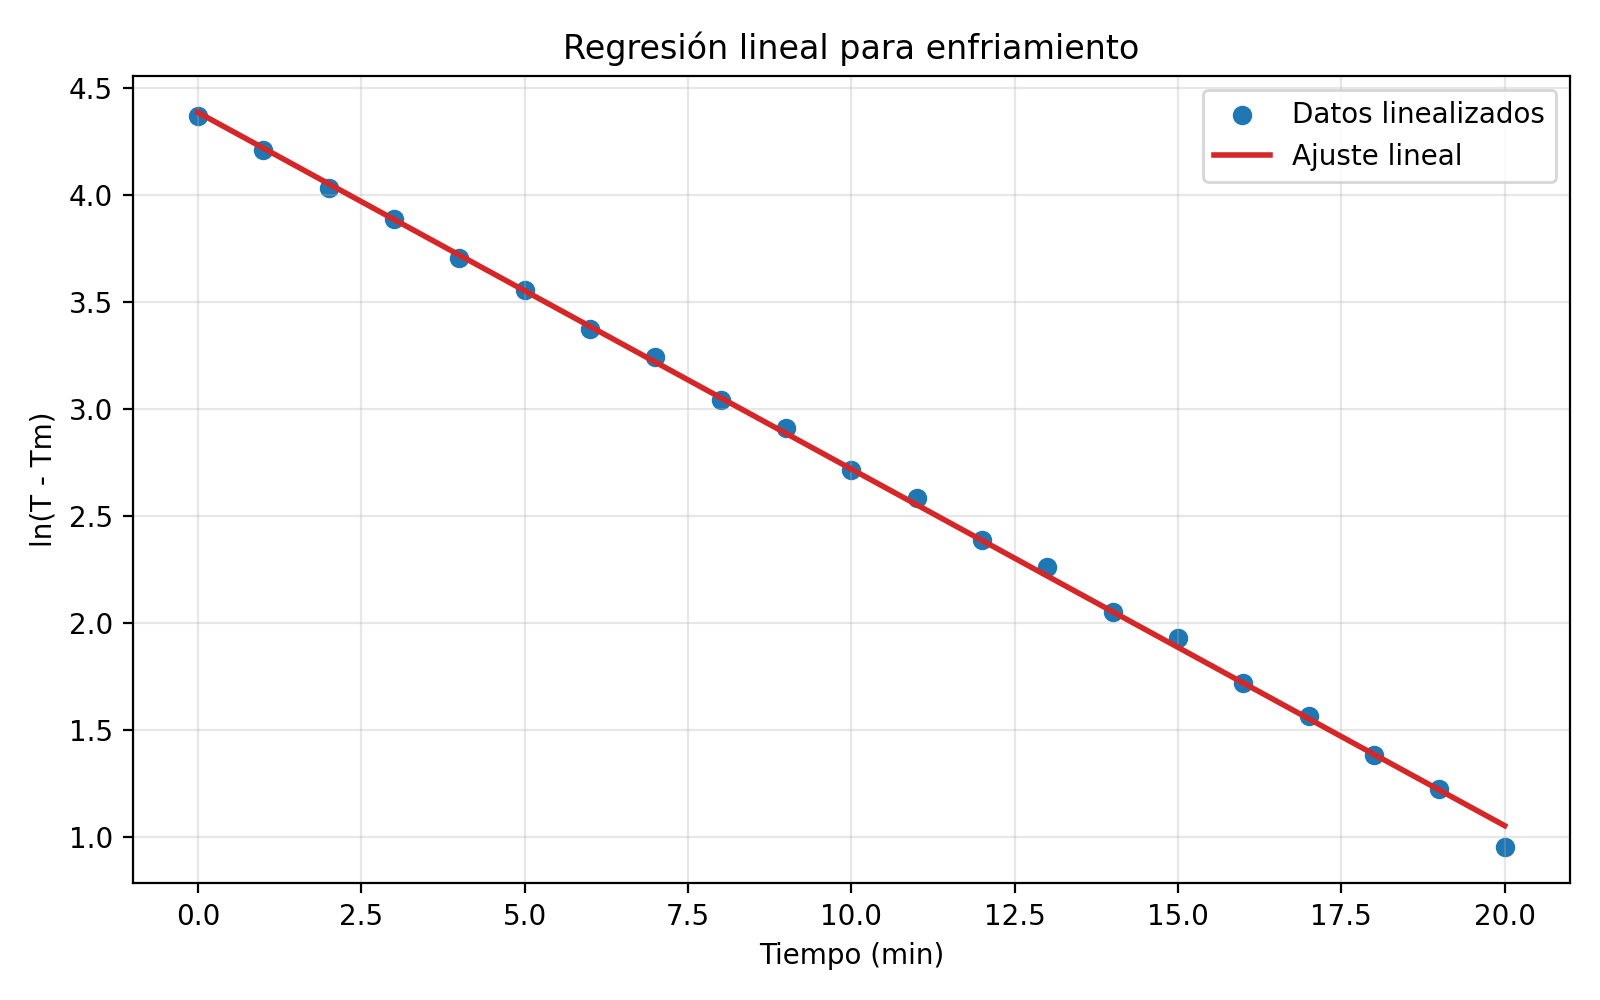
\includegraphics[width=0.64\textwidth]{../output/regresion_lineal.png}
    \caption{Datos linealizados y recta obtenida por mínimos cuadrados.}
    \label{fig:regresion}
\end{figure}

Al regresar de la variable logarítmica a la temperatura, el modelo numérico queda

\begin{equation}
    \boxed{T_{\mathrm{num}}(t)=18+80.4793e^{-0.166700t}}.
    \label{eq:modelo-numerico}
\end{equation}

Sustituimos la temperatura segura para encontrar el tiempo de cruce:

\begin{equation*}
    t_{\mathrm{num}}
    =\frac{\ln(27-18)-4.388000}{-0.166700}
    \approx 13.14\ \text{minutos}.
\end{equation*}

\subsection{Comprobación analítica y comparación}

Para comprobar el cálculo sin depender únicamente de la regresión, resolvemos la Ecuación~\eqref{eq:newton} con la condición inicial exacta. Como \(k>0\) y durante el proceso \(T>\Tamb\), el lado derecho es negativo; el modelo sí representa una pieza que se está enfriando. La ecuación es separable \citep{boyce2021,zill2018}:

\begin{align*}
    \frac{dT}{T-\Tamb} &= -k\,dt, \\
    \int\frac{dT}{T-\Tamb} &= \int-k\,dt, \\
    \ln\left|T-\Tamb\right| &= -kt+C_1, \\
    T(t) &= \Tamb+Ce^{-kt}.
\end{align*}

Podemos retirar el valor absoluto porque la pieza permanece por encima de \(18\,^{\circ}\mathrm{C}\) en el intervalo estudiado. Al aplicar \(T(0)=97\,^{\circ}\mathrm{C}\), la constante ya no se ajusta con todos los datos, sino que queda fijada por la medición inicial:

\begin{equation*}
    C=T(0)-\Tamb=97-18=79\,^{\circ}\mathrm{C}.
\end{equation*}

Conservamos \(k=0.166700\,\mathrm{min}^{-1}\), porque ese es el coeficiente que obtuvimos de los datos. La solución particular es

\begin{equation}
    \boxed{T_{\text{analítico}}(t)=18+79e^{-0.166700t}}.
    \label{eq:modelo-analitico}
\end{equation}

\begin{align*}
    27 &= 18+79e^{-0.166700t}, \\
    \frac{9}{79} &= e^{-0.166700t}, \\
    t_{\text{analítico}}
       &=\frac{\ln(9/79)}{-0.166700}
       \approx 13.03\ \text{minutos}.
\end{align*}

El resultado obtenido mediante la regresión es de \(13.14\) minutos, y la comprobación analítica da \(13.03\) minutos. La diferencia es

\begin{equation*}
    \Delta t=|13.14-13.03|=0.11\ \text{min}\approx6.6\ \text{s},
\end{equation*}

equivalente al \(0.84\,\%\) del tiempo analítico. La diferencia aparece principalmente porque la regresión ajusta tanto la pendiente como la intersección para acercarse a los 21 datos y obtiene \(C_{\mathrm{num}}=80.4793\,^{\circ}\mathrm{C}\). En la comprobación fijamos \(C=79\,^{\circ}\mathrm{C}\) para respetar exactamente \(T(0)=97\,^{\circ}\mathrm{C}\). El redondeo y la variación incluida en los datos simulados también afectan el ajuste.

Esta discrepancia no es un error de cálculo, sino una consecuencia de comparar dos modelos con distinto origen para cada constante. En el modelo analítico, \(C=79\,^{\circ}\mathrm{C}\) se deriva de forma exacta para satisfacer \(T(0)=97\,^{\circ}\mathrm{C}\). En el modelo numérico, en cambio, \(k=0.166700\,\mathrm{min}^{-1}\) proviene de la regresión, cuyo algoritmo ajusta simultáneamente pendiente e intersección para minimizar el error cuadrático global de las 21 mediciones; eso produce \(C_{\mathrm{num}}=80.4793\,^{\circ}\mathrm{C}\), equivalente a una temperatura inicial implícita de \(98.48\,^{\circ}\mathrm{C}\) en vez de los \(97\,^{\circ}\mathrm{C}\) reales. Para hacer que estos resultados sean compatibles, sería necesario forzar el intercepto de la regresión en \(b=\ln(97-18)=\ln(79)\) y ajustar solo la pendiente.

Cualitativamente, los dos modelos se comportan igual: la temperatura disminuye mientras \(T>18\,^{\circ}\mathrm{C}\), pero cada vez lo hace más despacio porque la diferencia térmica se reduce. Ambas soluciones se acercan a \(18\,^{\circ}\mathrm{C}\) sin seguir bajando indefinidamente por debajo del ambiente. Esa coincidencia, junto con la diferencia de solo 6.6 segundos, muestra que los resultados numérico y analítico son consistentes para estos datos.

\subsection{Cambio de temperatura ambiente a \texorpdfstring{\(24\,^{\circ}\mathrm{C}\)}{24 grados Celsius}}

Para estudiar el taller a \(24\,^{\circ}\mathrm{C}\), conservamos \(k=0.166700\,\mathrm{min}^{-1}\) como supuesto y cambiamos únicamente la temperatura del ambiente. Ahora la ecuación diferencial es

\begin{equation*}
    \frac{dT}{dt}=-0.166700(T-24).
\end{equation*}

Seguimos el mismo proceso de separación de variables y obtuvimos la solución general:

\begin{align*}
    \frac{dT}{T-24} &= -0.166700\,dt, \\
    \ln|T-24| &= -0.166700t+C_1, \\
    T(t) &= 24+Ce^{-0.166700t}.
\end{align*}

La condición inicial no cambia, de modo que

\begin{equation*}
    C=T(0)-24=97-24=73\,^{\circ}\mathrm{C}.
\end{equation*}

\begin{equation}
    \boxed{T(t)=24+73e^{-0.166700t}}.
    \label{eq:modelo-24}
\end{equation}

\begin{equation*}
    t=\frac{\ln(3/73)}{-0.166700}\approx19.15\ \text{minutos}.
\end{equation*}

Como se aprecia, el cambio no es trivial. Cerca de la temperatura segura, la pieza está apenas \(3\,^{\circ}\mathrm{C}\) por encima del nuevo dato de temperatura ambiente, en lugar de \(9\,^{\circ}\mathrm{C}\). Con una diferencia térmica menor, el enfriamiento se vuelve más lento antes de llegar a \(27\,^{\circ}\mathrm{C}\).

\begin{figure}[htbp]
    \centering
    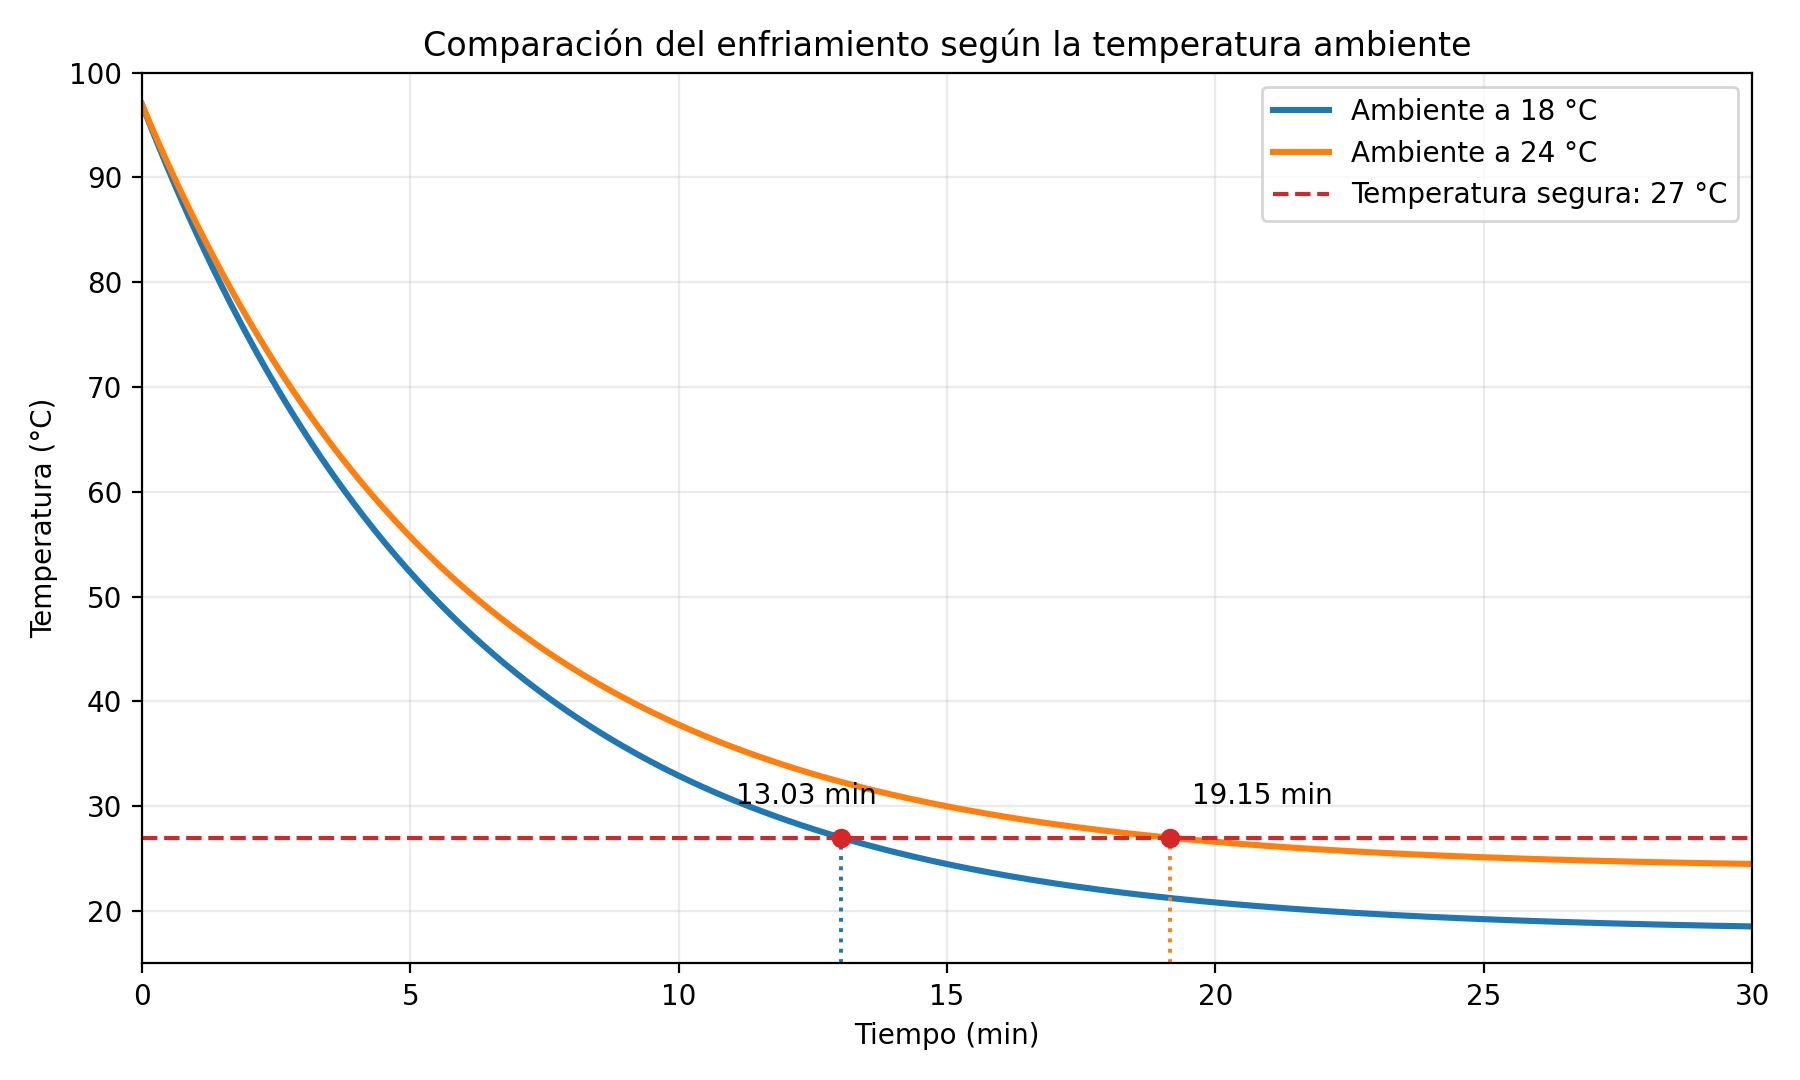
\includegraphics[width=0.72\textwidth]{../output/comparacion_escenarios.png}
    \caption{Curvas de temperatura para ambientes de \(18\,^{\circ}\mathrm{C}\) y \(24\,^{\circ}\mathrm{C}\). La línea roja marca \(27\,^{\circ}\mathrm{C}\).}
    \label{fig:comparacion-escenarios}
\end{figure}

En la Figura~\ref{fig:comparacion-escenarios} se aprecia el efecto sobre todo cerca del rango de \(27\,^{\circ}\mathrm{C}\): el caso de \(18\,^{\circ}\mathrm{C}\) la cruza a los \(13.03\) minutos y el de \(24\,^{\circ}\mathrm{C}\) a los \(19.15\) minutos. Bajo el supuesto de conservar \(k\), el cambio de ambiente añade \(6.12\) minutos.

Es importante destacar una limitación física en este escenario: bajo el supuesto matemático ideal de mantener \(k\) constante en \(0.1667\,\mathrm{min}^{-1}\), el tiempo obtenido es de \(19.15\) minutos. No obstante, en la realidad industrial, el coeficiente \(k\) no es enteramente independiente de la temperatura del entorno: varía por convección, de acuerdo con las propiedades físicas del material y del aire que lo rodea. Es razonable esperar que en un taller más caliente la \(k\) real sea ligeramente distinta a la calculada, por lo que \(19.15\) minutos representa en realidad un \textbf{límite inferior optimista}: la pieza real en el taller podría tardar algo más de tiempo en alcanzar la temperatura segura.

\section{Conclusión e interpretación}

En este estudio se determinó el coeficiente de enfriamiento del acero para los ejes de transmisión, bajo las condiciones específicas del taller, en \(k=0.166700\,\mathrm{min}^{-1}\). Con una temperatura ambiental de \(18\,^{\circ}\mathrm{C}\), el modelo de regresión lineal estimó un tiempo seguro de manipulación de \(13.14\) minutos (\(13\) min \(8\) s), mientras que la resolución exacta por separación de variables arrojó un tiempo de \(13.03\) minutos (\(13\) min \(2\) s).

A continuación se presenta la fundamentación analítica de estos resultados, organizada en tres ejes.

\subsection{Comportamiento asintótico y estado estable}

La solución analítica particular obtenida, \(T(t)=\Tamb+Ce^{-kt}\), describe el comportamiento térmico del sistema. Desde la teoría de ecuaciones diferenciales, el componente exponencial \(Ce^{-kt}\) funciona como el término transitorio del sistema, mientras que el parámetro constante \(\Tamb\) representa la solución de estado estable. Al evaluar el comportamiento asintótico mediante el límite cuando \(t\to\infty\), se observa que, dado que el coeficiente de enfriamiento es estrictamente positivo (\(k>0\)), la influencia de la condición inicial decae exponencialmente hasta anularse:
\[
\lim_{t\to\infty}\bigl(\Tamb+Ce^{-kt}\bigr)=\Tamb.
\]
Este límite matemático es consistente, a nivel físico (fuera del alcance de esta unidad de formación), con la Segunda Ley de la Termodinámica: garantiza que, dentro del modelo, la temperatura de la pieza no descenderá por debajo de la temperatura del ambiente que la rodea (\(18\,^{\circ}\mathrm{C}\) o \(24\,^{\circ}\mathrm{C}\), según el escenario).

\subsection{Origen de la diferencia entre el resultado numérico y el analítico}

La discrepancia de \(6.6\) segundos (\(\Delta t=0.11\) min) entre el enfoque numérico y el analítico se origina en el sesgo que introduce linealizar los datos antes de ajustarlos. Al aplicar mínimos cuadrados sobre la variable transformada \(y=\ln(T-\Tamb)\), el ajuste minimiza el error en la escala logarítmica y no en la escala térmica original. El modelo analítico, en cambio, impone con exactitud la condición inicial real de la pieza (\(C=T(0)-\Tamb=79\,^{\circ}\mathrm{C}\)), sacrificando el ajuste óptimo de los datos posteriores.

\subsection{Efecto de la temperatura ambiente sobre la rapidez de enfriamiento}

Al cambiar la temperatura del taller a \(24\,^{\circ}\mathrm{C}\), el tiempo necesario para alcanzar la temperatura segura de \(27\,^{\circ}\mathrm{C}\) aumenta a \(19.15\) minutos. Este incremento de \(6.12\) minutos se explica directamente a partir de la ecuación diferencial original,
\[
\frac{dT}{dt}=-k(T-\Tamb),
\]
donde la rapidez de enfriamiento es proporcional a la diferencia de temperaturas instantánea. Al acercarse la pieza a \(27\,^{\circ}\mathrm{C}\):

\begin{itemize}
    \item En el escenario de \(18\,^{\circ}\mathrm{C}\), la diferencia es \(27-18=9\,^{\circ}\mathrm{C}\).
    \item En el escenario de \(24\,^{\circ}\mathrm{C}\), la diferencia es \(27-24=3\,^{\circ}\mathrm{C}\).
\end{itemize}

En consecuencia, la magnitud de \(\left|\frac{dT}{dt}\right|\) al llegar a la temperatura segura es tres veces menor en el taller cálido que en el taller frío. Al ser la rapidez de cambio tres veces más lenta, la curva de temperatura para \(24\,^{\circ}\mathrm{C}\) se aplana de forma más pronunciada antes de alcanzar el objetivo, lo cual explica el retraso en el tiempo de enfriamiento.

\subsection{Limitaciones}

Para este ejercicio el modelo funciona bien, pero parte de datos simulados y supone una temperatura uniforme en todo el eje, un ambiente constante y un solo valor de \(k\). En una planta real habría que medir el proceso y revisar esos supuestos antes de fijar un tiempo seguro de manipulación.

\begin{thebibliography}{9}

\bibitem[Bergman et al.(2017)]{incropera2017}
Bergman, T. L., Lavine, A. S., Incropera, F. P., \& DeWitt, D. P. (2017).
\textit{Fundamentals of heat and mass transfer} (8th ed.). Wiley.

\bibitem[Boyce et al.(2021)]{boyce2021}
Boyce, W. E., DiPrima, R. C., \& Meade, D. B. (2021).
\textit{Elementary differential equations and boundary value problems} (12th ed.). Wiley.

\bibitem[Zill(2018)]{zill2018}
Zill, D. G. (2018).
\textit{Ecuaciones diferenciales con problemas con valores en la frontera} (9.\textsuperscript{a} ed.). Cengage Learning.

\end{thebibliography}

\end{document}